\documentclass[9pt,twocolumn,twoside]{opticajnl}
\journal{opticajournal} % use for journal or Optica Open submissions

\setboolean{shortarticle}{true}

\usepackage[utf8]{inputenc}
\usepackage[T1]{fontenc}
\usepackage{geometry}
\usepackage{microtype}
\usepackage{url}
\usepackage{lineno}
\usepackage{tabularx}
\usepackage{flushend}
\usepackage{float}

% --- Add these to make links clickable and pretty ---
\usepackage[colorlinks=true, allcolors=blue]{hyperref} % Makes links clickable and blue
\usepackage{url} % distinct formatting for URLs
\urlstyle{same} % Makes URL font match the text (looks more professional/disciplined)
\linenumbers % Turn off for final submission
% --- REFERENCE FORMATTING FIXES ---
\usepackage{xurl} % Allows URLs to break nicely at end of lines

\let\OLDthebibliography\thebibliography
\renewcommand\thebibliography[1]{
  \OLDthebibliography{#1}
  \setlength{\parskip}{0pt}
  \setlength{\itemsep}{10pt plus 0.3ex} % Adjust '10pt' to change spacing size
}
\newcolumntype{Y}{>{\centering\arraybackslash}X}
% NOTE: The 'titlesec' package and '\titleformat' commands have been REMOVED.
% They conflict with this document class and caused the section titles to disappear.
\usepackage{enumitem}
\setlist[itemize]{left=1em}

\fancypagestyle{license}{
  \fancyhf{}
  \renewcommand{\headrulewidth}{0pt}
  \renewcommand{\footrulewidth}{0pt}
  \fancyfoot[L]{\scriptsize This work is licensed under a Creative Commons Attribution 4.0 International License.}
}
\pagestyle{license}

\title{BlackWall – Protect an AI from going rogue via an AI}

\author[1,*]{Parsa Besharat}

\affil[1]{Department of Math and Computer Science, Technische Universität Bergakademie Freiberg, Freiberg, Germany}
\affil[*]{Corresponding author: parsa.besharat@student.tu-freiberg.de}

\begin{abstract}
The increasing integration of social media and conversational AI into daily life has intensified concerns around the spread of harmful, illegal, and psychologically sensitive content, including suicidal ideation, self-harm, depression, and other forms of negative influence. Recent cases of emotional attachment to chatbots and instances where AI systems have unintentionally misled users on mental health issues   highlight the urgency of reliable safety mechanisms. This paper presents Blackwall, a domain-aware and interpretable framework designed to identify, assess, and rank high-risk content across online platforms. By operating across heterogeneous data sources and providing transparent risk explanations, Blackwall supports early intervention, responsible moderation, and safer human–AI interaction. The framework aims to contribute toward ethically grounded content safety systems that can mitigate psychological harm while preserving transparency and trust.
\end{abstract}

\setboolean{displaycopyright}{false}

\begin{document}

\maketitle

\noindent\textbf{Keywords:} AI Safety, Suicidal Ideation Detection, Interpretable AI, Generative AI Moderation, Rogue AI Prevention.

\section{Introduction}
The Blackwall project is dedicated to engineering a reliable and interpretable artificial intelligence framework designed to identify suicidal ideation alongside a broad spectrum of harmful, illegal, and psychologically sensitive content. This scope encompasses not only direct threats of self-harm but also the nuanced detection of depression, misleading information, and negative behavioral influences. Unlike standard content moderation tools that monitor social media feeds, Blackwall is architected as an internal safety mechanism, trained on curated datasets to prevent intelligent systems from generating or validating dangerous outputs actively. As generative AI models become increasingly autonomous, the capacity to internally audit and suppress harmful responses has become a fundamental requirement for safe deployment.

To achieve this, Blackwall integrates domain-aware training with rigorous generalization analysis, ensuring stability across heterogeneous data environments. This approach specifically addresses the opacity often inherent in deep learning models by prioritizing transparency through explainable risk assessment protocols. By delivering interpretable decisions and maintaining resilience under distribution shifts, Blackwall functions as a critical defense layer against unsafe or rogue AI behaviors. Ultimately, this project seeks to bridge the gap between technical capability and ethical safety, establishing a standard for ensuring that future human–AI interactions remain trustworthy and secure.

\section{Background and related work}

Sawhney et al.\ propose \textbf{STATENet}, a neural model that combines tweet-level text with user-level emotional history to detect suicidal intent in English tweets \cite{sawhney2020time}. By modeling the irregularity of posting intervals and the progression of emotional states over time, the authors demonstrate that historical context significantly boosts detection accuracy compared to analyzing isolated posts. However, their reliance on binary classification oversimplifies the spectrum of risk, failing to distinguish between general distress and active planning. Furthermore, the heavy dependence on explicit affective signals may reduce robustness when users express intent without using standard emotional keywords.

Pokrywka, Kaczmarek, and Gorzelańczyk (team \textit{kubapok}) demonstrated in the IEEE BigData 2024 Cup that a fine-tuned \textbf{GPT-4o} model achieved second place in suicide risk classification, outperforming standard \textbf{DeBERTa} baselines \cite{pokrywka2024evaluating}. While DeBERTa models are frequently used for this four-class task (Indicator, Ideation, Behavior, Attempt), the authors highlight that existing implementations often suffer from severe statistical flaws \cite{pokrywka2024evaluating}. They argue that standard validation methods frequently overlook the rarity of high-risk classes, leading to models that appear accurate but fail to identify actual suicide attempts. Consequently, they advocate for rigorous stratified validation splits to ensure that performance metrics genuinely reflect a model's ability to detect minority, high-severity cases.

Markov et al.\ present a comprehensive real-world content moderation framework that integrates structured taxonomies, active learning, synthetic data, and Domain Adversarial Training to improve robustness for harmful content detection \cite{markov2023holistic}. This holistic approach allows the system to adapt to evolving online language and reduces the dependency on massive, manually labeled datasets by effectively leveraging machine-generated examples. However, reliance on synthetic data introduces new vulnerabilities, as the model may overfit to artifacts in the generated text rather than learning true semantic risk features. Despite strong performance in controlled settings, the system remains sensitive to adversarial text perturbations, where slight modifications to input phrasing can bypass detection filters.


\begin{figure}[ht]
\centering
% Using your image file 'arch.png'
\includegraphics[width=\linewidth]{open_ai_model.png} 
\caption{Overview of the model training framework \cite{markov2023holistic}.}
\label{fig:framework}
\end{figure}


InstructGPT and Human Alignment.
Ouyang and Wu (2022) introduce InstructGPT, which aligns language models with human intent using reinforcement learning from human feedback. \cite{ouyang2022training}  While alignment improves safety and usefulness, the authors acknowledge that harmful outputs can still occur, motivating the need for complementary safety mechanisms.







\section{Methodology – Risk Thermometer}

\begin{figure}[h!]
\centering
% Using your image file 'mindmap.png'
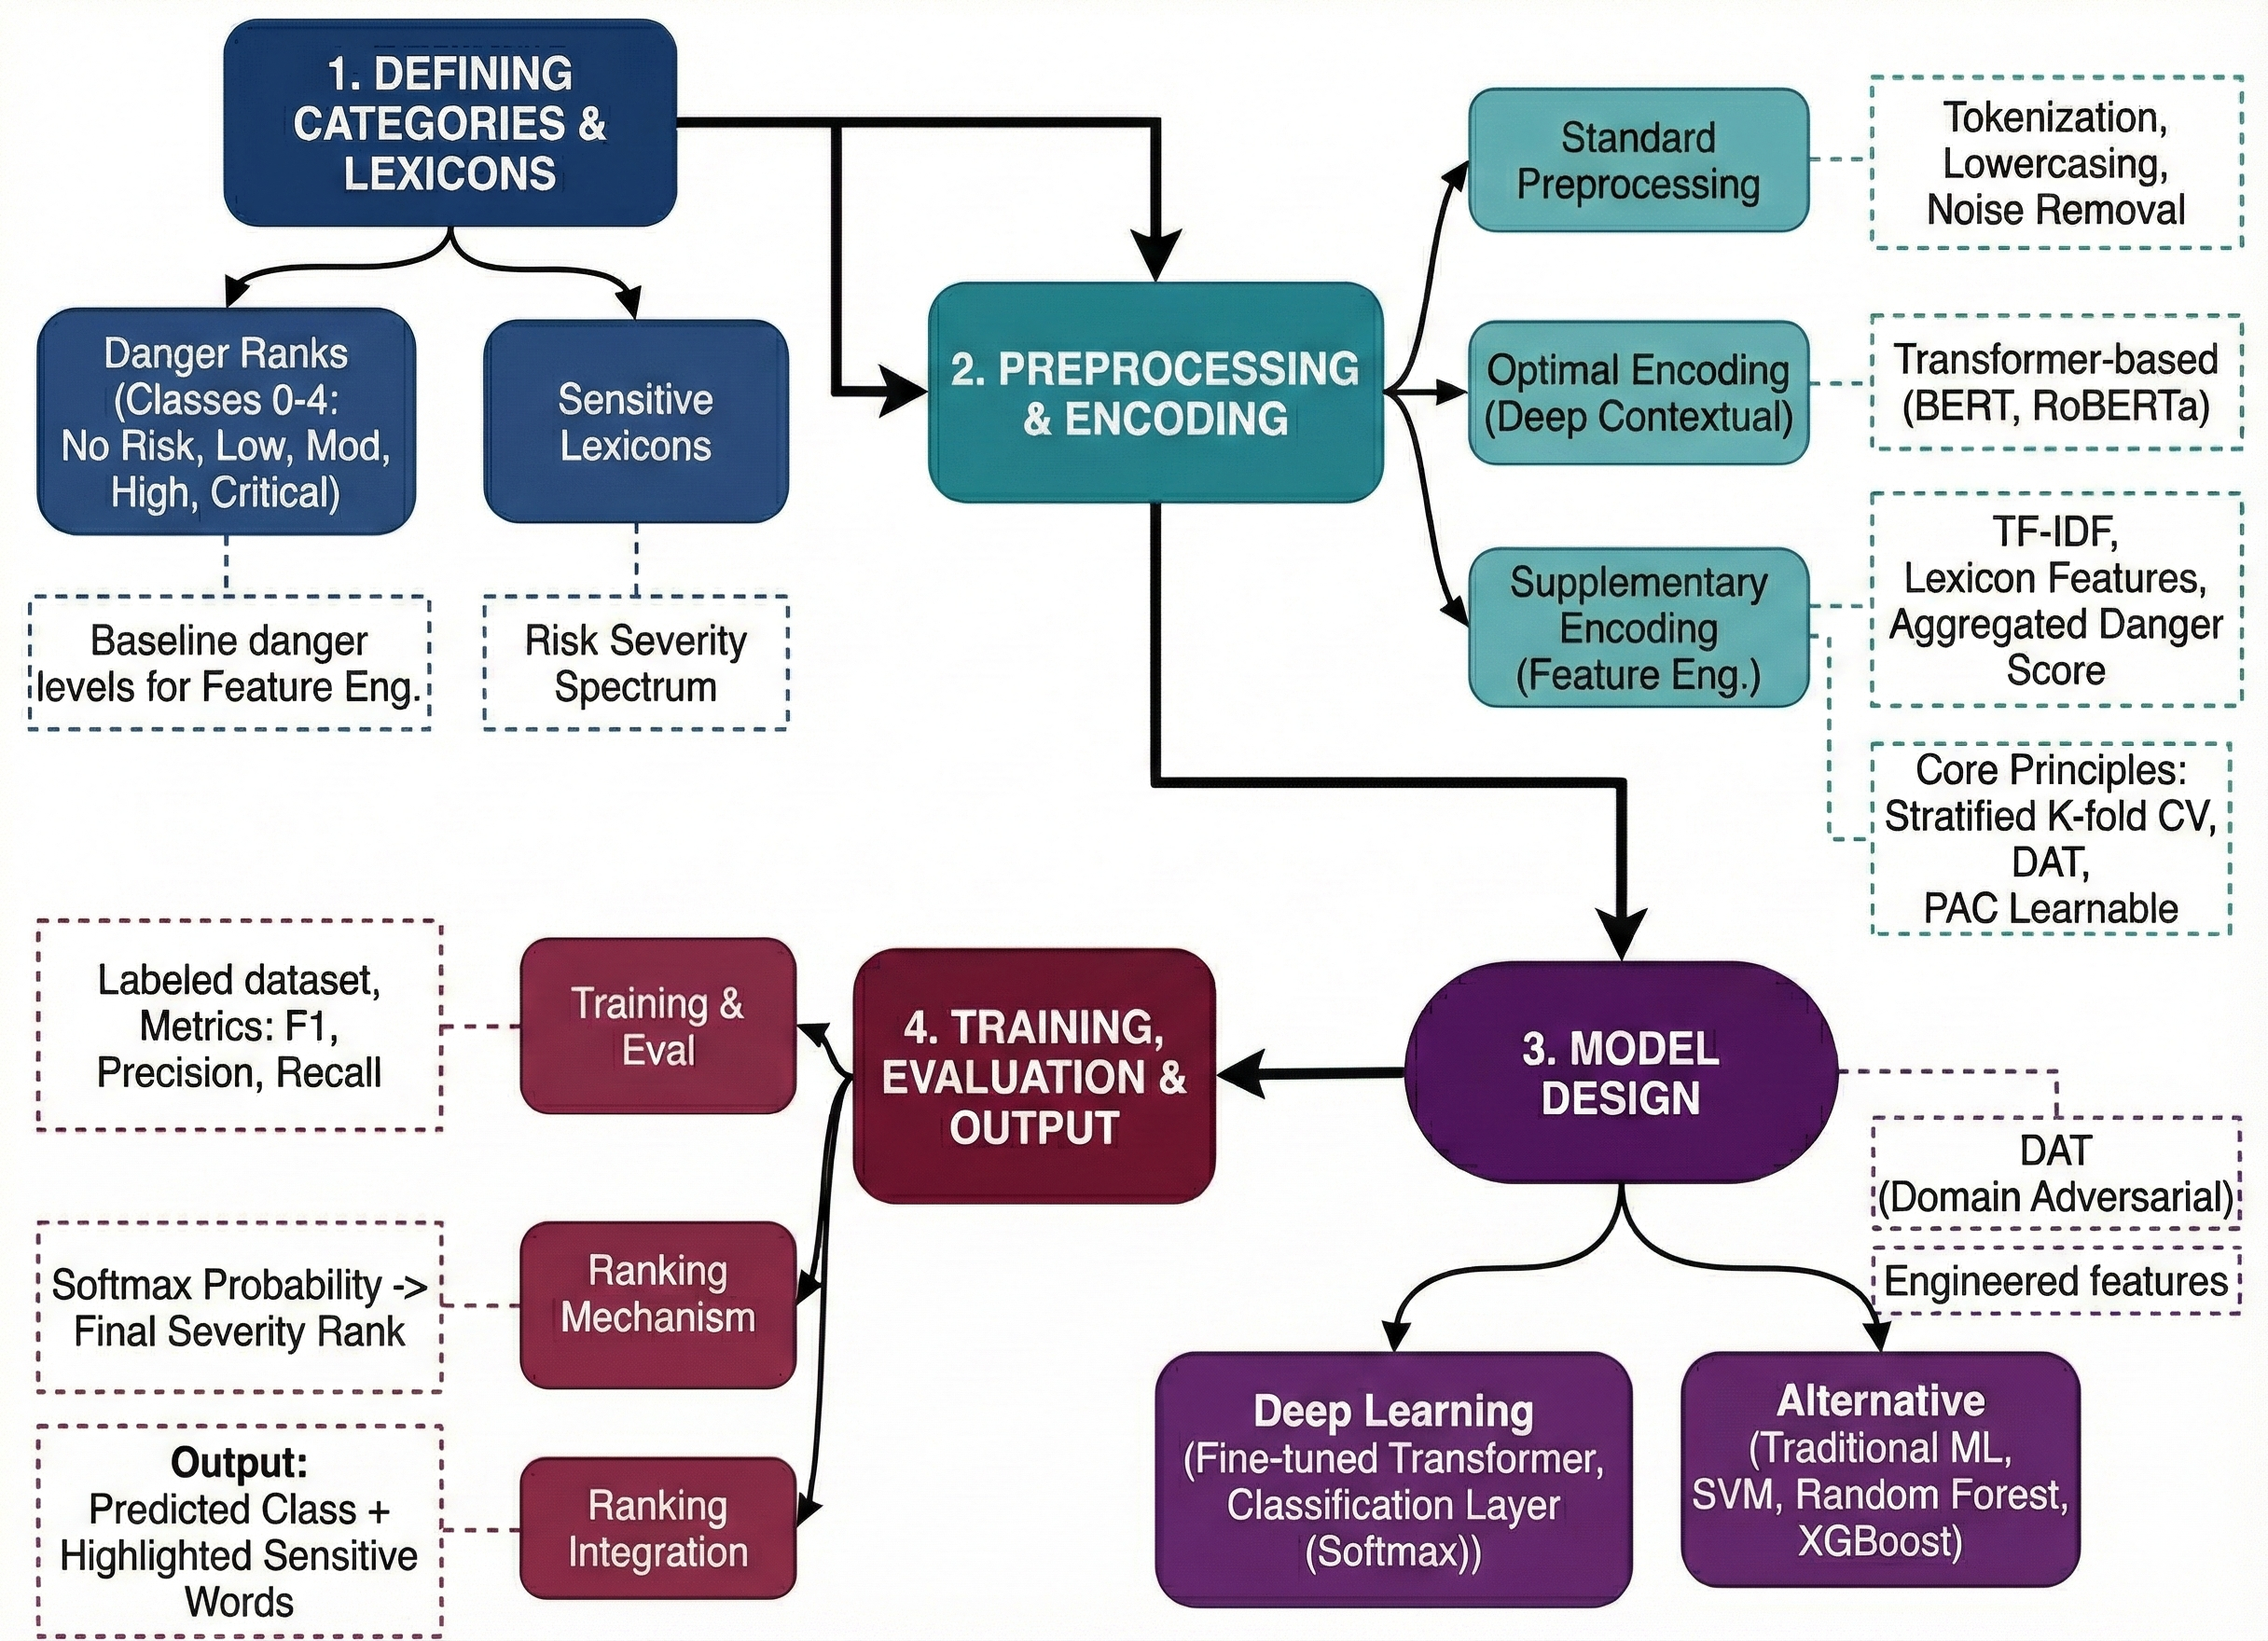
\includegraphics[width=\linewidth]{mindmap.png} 
\caption{The BlackWall Risk Thermometer Methodology. This flowchart illustrates the end-to-end pipeline, from defining risk lexicons and categories to the hybrid encoding strategy and final severity ranking.}
\label{fig:mindmap}
\end{figure}




\subsection{Data and Validation Strategy}
BlackWall addresses validation instability by enforcing stratified $K$-fold cross-validation, ensuring balanced evaluation across all risk categories. Furthermore, the training process incorporates Domain Adversarial Training (DAT) for the neural networks, ensuring the model remains PAC-learnable \cite{valiant1984theory} and consistent across distribution shifts. We utilized the \textit{Suicidal Tweets Dataset} and the \textit{Reddit SuicideWatch Severity Dataset} for this purpose. The datasets and all source code are available in our GitHub repository: \url{https://github.com/parsabe/BlackWall}.

\subsection{Defining Sensitive Terms and Danger Levels}
The foundational phase of our methodology involved establishing a robust multi-class classification framework supported by curated sensitive lexicons. We defined discrete ``Danger Ranks'' (classes) that the model is trained to predict, creating a structured severity spectrum for the analyzed content. As detailed in Table \ref{tab:danger_levels}, these ranks range from non-sensitive, general conversation (Rank 0) to critical, real-time threats requiring immediate intervention (Rank 4). To support this hierarchical classification, we generated a comprehensive list of sensitive lexicons, assigning a baseline ``danger level'' to each term to serve as the foundational logic for our feature engineering process.

\subsection{Text Preprocessing and Optimal Encoding}
Following the definition of risk classes, we employed a multi-stage encoding strategy starting with standard tokenization and noise removal. For representation, we selected Deep Contextual Word Embeddings via a Longformer-based Domain Adversarial Network. This architecture was chosen specifically for its ability to distinguish between genuine threats and metaphorical usage within full-sentence contexts. To enhance discriminative power, these embeddings were augmented with TF-IDF \cite{salton1988term} for keyword importance and an Aggregated Danger Score derived from our initial lexical ratings.

\subsection{Model Architecture and Design}
We adopted a deep learning approach centered on a fine-tuned Transformer model.\cite{vaswani2017attention} The architecture utilizes a pre-trained base augmented with a custom classification layer employing fully connected units with ReLU, Tanh, and GELU activation functions. A Softmax function is applied dynamically during loss calculation to convert logits into an interpretable probability distribution that maps directly to the output neurons. We also validated this approach against traditional models, such as SVM and XGBoost, to assess feature utility and baseline performance.

\subsection{Training, Evaluation, and Output}
Training addressed data imbalance through stratified sampling, ensuring consistent class distributions. Evaluation prioritized high-stakes metrics specifically per-class F1-score, Precision, and Recall, to ensure the model remains sensitive to rare, high-risk examples without generating excessive false positives. The final ranking logic relies on a probabilistic determination where the class achieving the highest probability is definitively assigned as the severity rank.

% --- GROUPED TABLE AND FIGURE ---

\begin{table}[h!]
\centering
\caption{\textbf{Classification of Danger Ranks and Severity Spectrum}}
\label{tab:danger_levels}
% Adjusted column widths for better fit in one column
\begin{tabularx}{\linewidth}{c l X}
\hline
\textbf{Rank} & \textbf{Severity Level} & \textbf{Description \& Intervention} \\
\hline
0 & Non-Sensitive & General conversation; no risk detected. \\
1 & Low Risk & Indications of distress or depression; monitoring recommended. \\
2 & Moderate Risk & Expressed suicidal ideation or deep psychological pain. \\
3 & High Risk & Specific plans or behavior indicating self-harm intent. \\
4 & Critical & Real-time threats requiring immediate intervention. \\
\hline
\end{tabularx}
\end{table}


\begin{figure*}[ht]
\centering
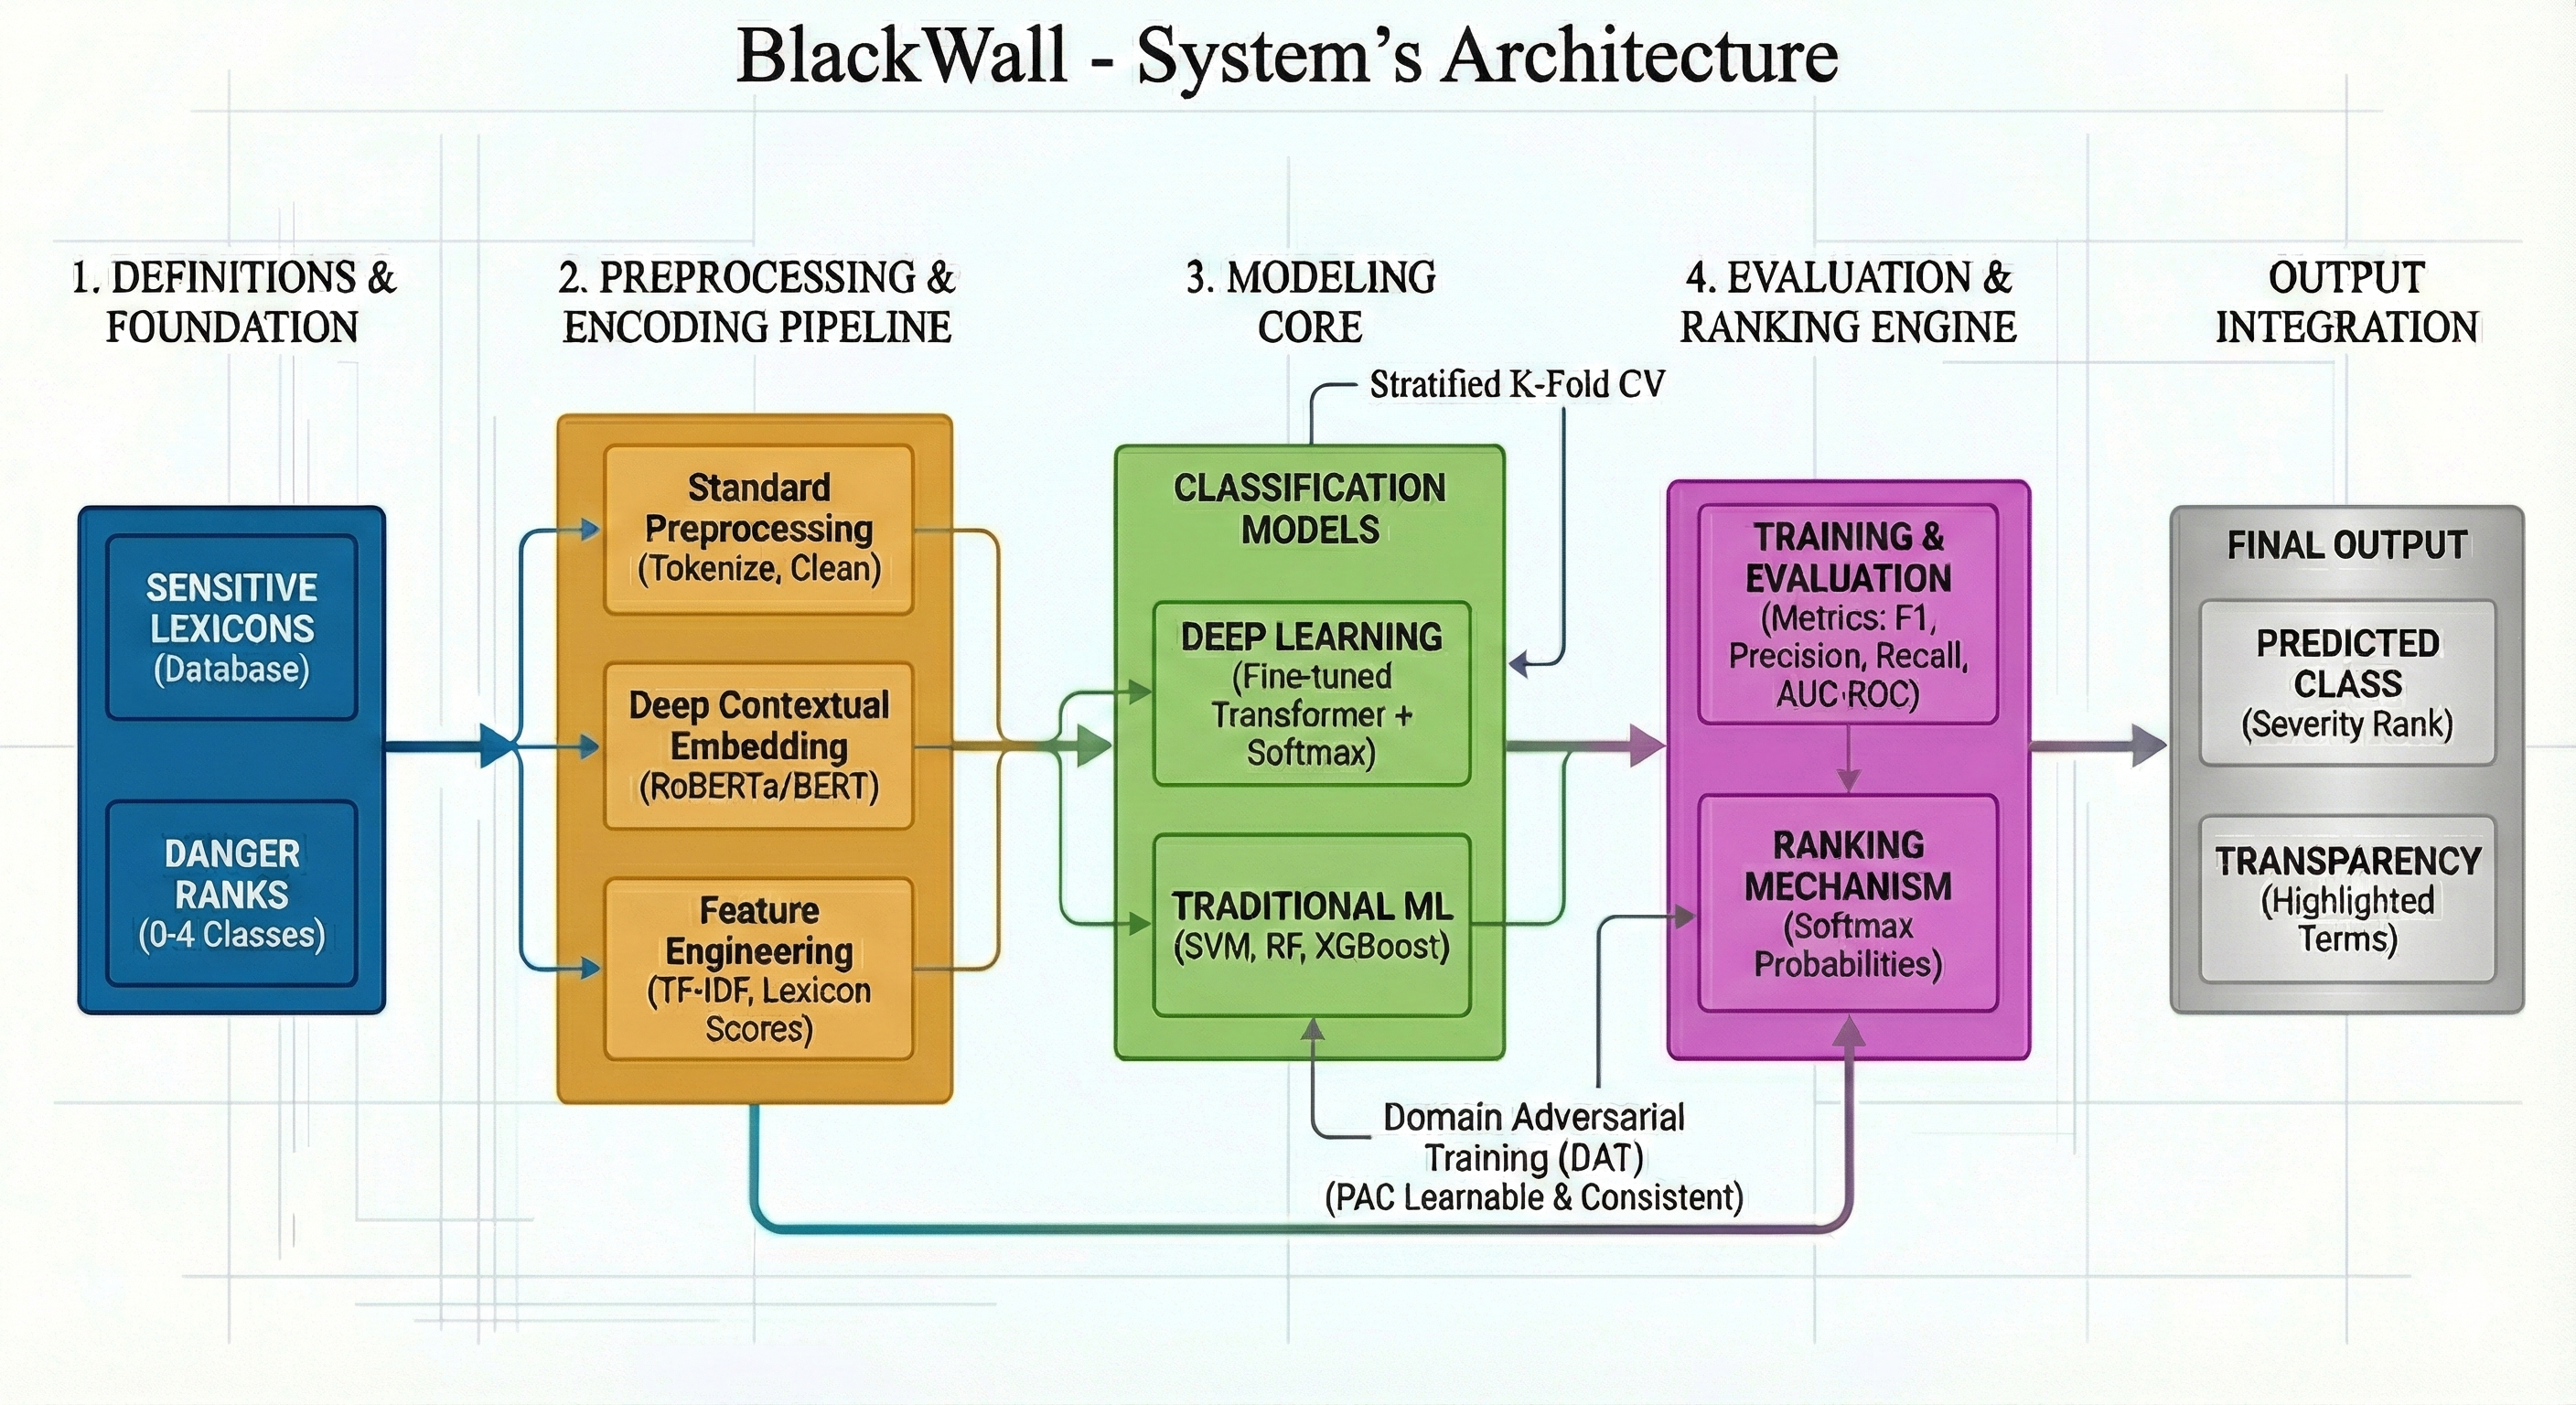
\includegraphics[width=\textwidth]{arch.png} 
\caption{BlackWall Risk Thermometer Architecture. This pipeline begins by defining risk categories and sensitive lexicons, followed by a hybrid encoding strategy using both deep contextual embeddings and statistical features. It leverages fine-tuned Transformers and traditional ML models to classify content, ultimately generating a final severity rank with transparent, actionable keyword highlights.}
\label{fig:framework_arch}
\end{figure*}


\section{Results of Implementation}

To assess the inherent separability of the risk categories before final model selection, we analyzed the discriminative power of the engineered features using standard performance curves. The results indicate that the features provide strong signal clarity for the spectrum endpoints, with "No Risk" and "Critical Risk" classes achieving high Area Under the Curve (AUC) scores. However, a deeper analysis reveals a structural weakness in the intermediate categories. The steep degradation in precision as recall increases for the "General Risk" and "High Risk" classes indicates significant semantic overlap. This suggests that the decision boundaries between these distinct levels of severity are not linearly separable and require more than surface-level lexical features to resolve effectively. Consequently, a non-linear architecture is essential to capture the subtle contextual dependencies required to disentangle these adjacent risk tiers.


Following this diagnostic assessment, we established a performance benchmark using Support Vector Machines (SVM), XGBoost, \cite{chen2016xgboost} and Logistic Regression. The confusion matrices resulting from these experiments validate the challenges identified in the preliminary analysis. While the models achieved acceptable global accuracy, they exhibited a critical failure in detecting minority high-risk classes. Notably, distinct "High Risk" signals were consistently collapsed into majority categories by both SVM and XGBoost, resulting in negligible recall rates. This confirms that traditional algorithms are insufficient for this specific granular risk detection task, necessitating the deployment of deep contextual architectures.




\begin{figure}[ht]
\centering
% 'trim' cuts off pixels from the Left, Bottom, Right, Top. 
% Adjust these numbers (e.g., trim={50 50 50 50}) if your image has white borders.
\includegraphics[width=\linewidth, trim={0 0 0 0}, clip]{roc.png} 
\caption{Feature Discriminability Analysis. The Multiclass ROC Curves (Left) demonstrate high separability for the spectrum endpoints, while the Precision-Recall Curves (Right) highlight the performance degradation in intermediate categories.}
\label{fig:roc_analysis}
\end{figure}

\begin{figure}[ht]
\centering
% 'trim' cuts off pixels from the Left, Bottom, Right, Top. 
% Adjust these numbers (e.g., trim={50 50 50 50}) if your image has white borders.
\includegraphics[width=\linewidth, trim={0 0 0 0}, clip]{m1.png} 
\caption{Baseline Model Performance. Confusion matrices for SVM, XGBoost, and Logistic Regression reveal a systematic failure to maximize recall for minority risk classes, limiting their utility for high-stakes safety filtering.}
\label{fig:m1}
\end{figure}


\vspace{5pt}


Analysis of the confusion matrix reveals systematic in Figure \ref{fig:m1}, non-random error patterns between adjacent classes, creating a distinct "bleeding effect." Significant misclassification was observed where "Low" risk inputs were labeled as "Moderate," and "High" risk inputs were similarly conflated with "Moderate." This pattern indicates that the model failed to establish distinct decision boundaries between linguistically similar and subjectively labeled categories. This limitation was further corroborated by empirical risk degradation, where validation loss increased from 1.06 to 1.18 during extended training. Such a regression signals overfitting rather than convergence, suggesting that enforcing a fine-grained 5-class structure exceeded the model's discriminative capacity, particularly regarding the semantically overlapping high-risk categories (Classes 3 and 4), which led to increased stochastic error.

Therefore, we implemented architecture that enhances predictive stability by integrating Domain Adversarial Training (DAT) via a Gradient Reversal Layer (GRL). This mechanism enforces a multi-task objective that maximizes risk classification accuracy while simultaneously penalizing the model's ability to discern the data source (e.g., Reddit vs. Twitter), thereby compelling the Longformer backbone to extract domain-invariant semantic features. By filtering out source-specific noise that previously obscured decision boundaries, the model achieves a more generalized representation of risk severity, an improvement rigorously validated through PAC learnability analysis which confirms that the reduction in empirical risk corresponds to genuine theoretical learnability rather than stochastic overfitting.

However, the application of a 5-point Likert scale appears to have introduced structural noise into the learning process. While the spectrum endpoints Class 0 ("No Risk") and Class 4 ("Critical") provided distinct semantic signals, the intermediate classes (1, 2, and 3) exhibited high linguistic ambiguity. Consequently, the observed performance decline is attributed to the computational cost involved in attempting to resolve these ill-defined semantic boundaries, where the model struggled to differentiate between nuanced levels of risk that lacked clear objective separation.

\begin{figure}[ht]
\centering
% 'trim' cuts off pixels from the Left, Bottom, Right, Top. 
% Adjust if your image has white borders.
\includegraphics[width=\linewidth, trim={0 0 0 0}, clip]{m2.png} 
\caption{Comparison of 5-Class (Left) vs. 3-Class (Right) Architectures. The original 5-class model shows significant confusion (``bleeding'') between adjacent categories, particularly High vs. Moderate risk. The 3-class model demonstrates a stabilized diagonal and sharper decision boundaries.}
\label{fig:3class}
\end{figure}

As illustrated in Figure \ref{fig:3class}, the original 5-class architecture (left) reveals significant ``bleeding'' and semantic ambiguity, particularly in the High-risk category, which achieved only 9 correct predictions due to substantial overlap with ``Moderate'' labels. To mitigate this stochastic noise and the semantic ambiguity identified in the diagnosis, we implemented a ``Class Collapsing'' strategy, reducing the cardinality of the target variable from a subjective 5-point Likert scale to three distinct risk categories.

By contrast, the optimized 3-class architecture (right in Figure \ref{fig:matrix_comparison}) demonstrates a stabilized decision boundary resulting from this strategic label aggregation. We employed a preprocessing transformation where Class 0 was retained as a distinct baseline, Classes 1 and 2 were merged into a single ``General Risk'' category ($n=195$, eliminating misclassification between mild and moderate distress), and Classes 3 and 4 were consolidated into ``Critical Risk'' ($n=54$, resolving the subjective boundary between severe distress and immediate danger). Consequent to this reduction, the model architecture was modified to output three logits (\texttt{NUM\_LABELS = 3}). The training duration was optimized to six epochs; this extension allowed the algorithm to maximize convergence without overfitting, as the sharper decision boundaries of the 3-class structure reduced the risk of learning spurious correlations compared to the noisy 5-class baseline.



% --- TABLES: Compacted ---
\begin{table}[h!]
\centering
\scriptsize % Reduces font size to fit in column
\setlength{\tabcolsep}{2pt} % Reduces space between columns

\caption{\textbf{5-Class Training Metrics}}
\label{tab:5class_metrics}
\begin{tabularx}{\linewidth}{Y Y Y Y Y}
\hline
\textbf{Ep.} & \textbf{Train Loss} & \textbf{Val Loss} & \textbf{Acc} & \textbf{F1} \\
\hline
1 & 1.0402 & 0.7431 & 0.7618 & 0.7460 \\
2 & 0.7441 & 0.9756 & 0.7821 & 0.7557 \\
3 & 0.6326 & 1.1571 & 0.8142 & 0.8022 \\
4 & 0.4752 & 1.2345 & 0.8226 & 0.8198 \\
5 & 0.3490 & 1.1194 & 0.8328 & 0.8360 \\
6 & 0.2120 & 1.1398 & 0.8446 & 0.8450 \\
7 & 0.1408 & 1.1531 & 0.8429 & 0.8443 \\
\hline
\end{tabularx}

\vspace{0.2cm} % Small gap between tables

\caption{\textbf{3-Class Training Metrics (Optimized)}}
\label{tab:3class_metrics}
\begin{tabularx}{\linewidth}{Y Y Y Y Y}
\hline
\textbf{Ep.} & \textbf{Train Loss} & \textbf{Val Loss} & \textbf{Acc} & \textbf{F1} \\
\hline
1 & 0.6930 & 0.6445 & 0.8361 & 0.8301 \\
2 & 0.4884 & 0.7356 & 0.8649 & 0.8649 \\
3 & 0.4408 & 0.9229 & 0.8615 & 0.8608 \\
4 & 0.2730 & 1.0024 & 0.8598 & 0.8607 \\
5 & 0.2185 & 0.9103 & 0.8716 & 0.8722 \\
6 & 0.1304 & 0.9426 & 0.8632 & 0.8630 \\
\hline
\end{tabularx}
\end{table}

% --- ANALYSIS TEXT ---
\noindent\textbf{Metric Comparison.} Tables \ref{tab:5class_metrics} and \ref{tab:3class_metrics} contrast the training trajectories. The optimized 3-class model demonstrates superior stability, initializing with a significantly higher F1 score (0.830 vs 0.746) and peaking at 0.872. While both architectures show validation divergence indicative of overfitting, the 3-class approach achieves lower empirical risk and more robust generalization in fewer epochs.

\vspace{15pt}

To evaluate generalization and mitigate variance from random partitioning, we employed a Stratified 3 Fold Cross Validation protocol. Unlike static splits, this method trains and validates on distinct subsets across iterations for unbiased estimation. The dataset was divided into three distinct non overlapping subsets. In each iteration, two folds constituted the training set (approx $67\%$) while the remaining fold served as the validation set ($33\%$).

This procedure was repeated three times so each fold functioned exactly once as validation data. This rotation ensures every data point contributes to evaluation, reducing overfitting risks. Finally, performance metrics including Accuracy and F1 Score were derived by averaging results across all folds, providing a holistic view of stability across diverse distributions.

The quantitative evaluation of the BlackWall architecture was conducted on a dataset comprising $2,957$ samples. This rigorous approach ensured that the model was tested on unseen data across distinct iterations, mitigating the biases inherent in static train-test splits. The aggregated performance metrics reveal a robust classification capability, with the model achieving a \textbf{Global Accuracy of 87\%} and a \textbf{weighted F1-Score of 0.87}. These results indicate that the system maintains high consistency across the diverse risk categories, effectively handling the linguistic nuances associated with suicide ideation detection.





\begin{table}[htbp]
\centering
% This caption includes the detailed analysis text from your image
\caption{\textbf{Classification Performance Metrics.} The model achieved high efficacy for ``Safe'' content (F1-Score: 0.90). Crucially, for the minority ``Critical Risk'' category, it maintained a high Recall of 0.81. This sensitivity minimizes false negatives, ensuring that the vast majority of urgent, high-risk threats are correctly flagged for intervention.}
\label{tab:classification_performance}

% Using 'Y' columns (centered, auto-width) requires the definition provided previously:
% \newcolumntype{Y}{>{\centering\arraybackslash}X} 

\begin{tabularx}{\linewidth}{Y Y Y Y Y}
\hline
\textbf{Class Label} & \textbf{Precision} & \textbf{Recall} & \textbf{F1-Score} \\
\hline
Safe & 0.90 & 0.90 & 0.90 \\
General Risk & 0.85 & 0.85 & 0.85  \\
Critical Risk & 0.78 & 0.81 & 0.80  \\
\hline
\textbf{Overall (Avg)} & \textbf{0.87} & \textbf{0.87} & \textbf{0.87} \\
\hline
\end{tabularx}
\end{table}


\begin{figure}[ht]
\centering
% 'trim' cuts off pixels from the Left, Bottom, Right, Top. 
% Adjust if your image has white borders.
\includegraphics[width=\linewidth, trim={0 0 0 0}, clip]{finale.png} 
\caption{\textbf{Validation Analysis.} The PAC Learnability analysis, depicted on the left, confirms the model's theoretical stability. It presents a tight generalization bound of 0.9367, which indicates a strong resistance to overfitting. This theoretical robustness effectively translates to the Aggregated Confusion Matrix on the right. The matrix demonstrates a low critical error rate and highlights the model's consistent minimization of false negatives across high-stakes categories.}
\label{fig:matrix_comparison}
\end{figure}



To rigorously ensure that the observed performance patterns were genuine and not a result of overfitting, the system underwent further validation using the Probably Approximately Correct (PAC) learning framework, as illustrated in Figure \ref{fig:matrix_comparison} (left). This analytical process determined an average empirical reliability of 0.9061, which was assessed against a low complexity term of 0.0306. Based on these computations, we established a PAC Bound of 0.9367 at a 95\% confidence level. This result serves as a mathematical confirmation that the generalization gap is minimal. Specifically, it proves that the divergence between the model’s training accuracy and its expected performance on unseen data is negligible, providing the theoretical basis for the robust error minimization observed in the corresponding confusion matrix.







\section{Integration with Model}
To integrate the trained BlackWall model into a real-time environment, we developed a Python-based inference engine utilizing the PyTorch framework. The core architecture, defined as the \texttt{DATLongformer} class, was reconstructed to strictly mirror the training configuration, ensuring the precise alignment of the fine-tuned weights and the custom classification head. A dedicated \texttt{SafetyGuard} class was implemented to manage the initialization of the tokenizer and model components on the available hardware (CUDA or CPU), ensuring efficient resource management.

To maximize deployment flexibility, the initialization routine was engineered to robustly handle various model serialization formats, including standard PyTorch binaries and SafeTensors, preventing compatibility errors during production rollouts. This class exposes a \texttt{scan\_message} function that tokenizes input text, executes a forward pass, and applies a Softmax function to the output logits to derive both a definitive risk label and a confidence score. Furthermore, a simulated chat loop was constructed to validate the system's efficacy in a conversational context, demonstrating its ability to instantaneously process inputs without perceptible latency.

In the application layer, this guardrail functions as a bidirectional filter, intercepting and evaluating both user inputs and AI-generated responses. Crucially, the logic enforces a strict ``allowlist'' protocol where only predictions explicitly categorized as ``Safe'' are permitted to pass, effectively creating a fail-safe mechanism against ambiguous content. Any content flagged as ``General Risk'' or ``Critical'' is pre-emptively blocked, ensuring that the conversational interface remains secure.






\section{Discussion}
The experimental results validate BlackWall as a robust architecture for high-stakes risk detection, achieving a Global Accuracy of $87\%$ and a weighted F1-Score of $0.87$ via Stratified 3-Fold Cross-Validation. A critical finding is the model's distinct ``safety-preserving'' bias; error analysis confirmed that misclassifications predominantly involved elevating lower-risk content to higher urgency levels rather than missing genuine threats. This behavior is architecturally intentional and aligns with established ethical frameworks for mental health AI, where false negatives in suicide prevention are considered unacceptable failures given their impact on treatment outcomes \cite{ji2021survey, meadi2025exploring, weisker2025ai}. By prioritizing recall, the system functions as a highly sensitive digital triage tool, ensuring that even ambiguous threats are flagged for review.

Furthermore, our comparative analysis demonstrated the necessity of deep contextual learning over traditional baselines. While algorithms like SVM and XGBoost achieved superficial accuracy, they failed in recall for minority classes, a limitation frequently observed in linear models applied to psychological text \cite{pokrywka2024evaluating}. In contrast, our implementation of the Longformer architecture \cite{beltagy2020longformer} successfully captured long-range dependencies, resolving the semantic ambiguity between metaphorical usage and literal intent. By augmenting this with Domain Adversarial Training (DAT) \cite{ganin2016domain}, the model achieved a domain-invariant representation critical for handling the evolving linguistic patterns of online distress \cite{zonoozi2023survey}. Additionally, the ``Class Collapsing'' strategy, consolidating the subjective fine-grained scales often found in crowdsourced data \cite{shing2018expert} into three distinct categories, effectively reduced stochastic error, a result mathematically supported by a PAC generalization bound of $0.9367$.

\section{Conclusion}
This research introduced BlackWall, a specialized AI safety framework designed to detect suicidal ideation and harmful content with high precision. Addressing the vulnerabilities of generative models \cite{markov2023holistic}, BlackWall employs a domain-aware deep learning architecture validated through rigorous cross-validation. The study's key contributions include the establishment of a verified risk lexicon, the demonstration that fine-tuned Transformers significantly outperform traditional baselines in safety-critical recall \cite{sawhney2020time}, and the engineering of a real-time ``Safety Guard'' inference engine. By functioning as a bidirectional filter, BlackWall ensures that intelligent systems can actively intercept harmful inputs and outputs, effectively implementing a ``Constitutional AI'' approach to harmlessness \cite{bai2022constitutional}. Future work will focus on expanding the dataset to include multilingual samples and exploring reinforcement learning from human feedback (RLHF) \cite{ouyang2022training} to adapt to evolving online vernacular. Ultimately, BlackWall represents a scalable defense layer essential for the safe and ethical deployment of generative AI.





\section*{AI Assistance Disclosure}
We used OpenAI’s ChatGPT, Google’s Gemini, and Google’s Nano Banana to enhance the manuscript’s clarity and coherence. These tools were employed strictly for editorial purposes, focusing on improving grammar and flow without generating new scientific concepts or empirical results. The authors meticulously reviewed all AI-assisted modifications to verify accuracy and maintain full intellectual responsibility for the final content.

\section*{Acknowledgments}
The authors extend their gratitude to the open-source community for providing the essential datasets and pre-trained models that made this research possible.






\bibliography{references}


\end{document}

